\documentclass{ximera}

 

\usepackage{epsfig}

\graphicspath{
  {./}
  {figures/}
}

\usepackage{morewrites}
\makeatletter
\newcommand\subfile[1]{%
\renewcommand{\input}[1]{}%
\begingroup\skip@preamble\otherinput{#1}\endgroup\par\vspace{\topsep}
\let\input\otherinput}
\makeatother

\newcommand{\includeexercises}{\directlua{dofile("/home/jim/linearAlgebra/laode/exercises.lua")}}

%\newcounter{ccounter}
%\setcounter{ccounter}{1}
%\newcommand{\Chapter}[1]{\setcounter{chapter}{\arabic{ccounter}}\chapter{#1}\addtocounter{ccounter}{1}}

%\newcommand{\section}[1]{\section{#1}\setcounter{thm}{0}\setcounter{equation}{0}}

%\renewcommand{\theequation}{\arabic{chapter}.\arabic{section}.\arabic{equation}}
%\renewcommand{\thefigure}{\arabic{chapter}.\arabic{figure}}
%\renewcommand{\thetable}{\arabic{chapter}.\arabic{table}}

%\newcommand{\Sec}[2]{\section{#1}\markright{\arabic{ccounter}.\arabic{section}.#2}\setcounter{equation}{0}\setcounter{thm}{0}\setcounter{figure}{0}}

\newcommand{\Sec}[2]{\section{#1}}

\setcounter{secnumdepth}{2}
%\setcounter{secnumdepth}{1} 

%\newcounter{THM}
%\renewcommand{\theTHM}{\arabic{chapter}.\arabic{section}}

\newcommand{\trademark}{{R\!\!\!\!\!\bigcirc}}
%\newtheorem{exercise}{}

\newcommand{\dfield}{{\sf dfield9}}
\newcommand{\pplane}{{\sf pplane9}}

\newcommand{\EXER}{\section*{Exercises}}%\vspace*{0.2in}\hrule\small\setcounter{exercise}{0}}
\newcommand{\CEXER}{}%\vspace{0.08in}\begin{center}Computer Exercises\end{center}}
\newcommand{\TEXER}{} %\vspace{0.08in}\begin{center}Hand Exercises\end{center}}
\newcommand{\AEXER}{} %\vspace{0.08in}\begin{center}Hand Exercises\end{center}}

% BADBAD: \newcommand{\Bbb}{\bf}

\newcommand{\R}{\mbox{$\Bbb{R}$}}
\newcommand{\C}{\mbox{$\Bbb{C}$}}
\newcommand{\Z}{\mbox{$\Bbb{Z}$}}
\newcommand{\N}{\mbox{$\Bbb{N}$}}
\newcommand{\D}{\mbox{{\bf D}}}
\usepackage{amssymb}
%\newcommand{\qed}{\hfill\mbox{\raggedright$\square$} \vspace{1ex}}
%\newcommand{\proof}{\noindent {\bf Proof:} \hspace{0.1in}}

\newcommand{\setmin}{\;\mbox{--}\;}
\newcommand{\Matlab}{{M\small{AT\-LAB}} }
\newcommand{\Matlabp}{{M\small{AT\-LAB}}}
\newcommand{\computer}{\Matlab Instructions}
\newcommand{\half}{\mbox{$\frac{1}{2}$}}
\newcommand{\compose}{\raisebox{.15ex}{\mbox{{\scriptsize$\circ$}}}}
\newcommand{\AND}{\quad\mbox{and}\quad}
\newcommand{\vect}[2]{\left(\begin{array}{c} #1_1 \\ \vdots \\
 #1_{#2}\end{array}\right)}
\newcommand{\mattwo}[4]{\left(\begin{array}{rr} #1 & #2\\ #3
&#4\end{array}\right)}
\newcommand{\mattwoc}[4]{\left(\begin{array}{cc} #1 & #2\\ #3
&#4\end{array}\right)}
\newcommand{\vectwo}[2]{\left(\begin{array}{r} #1 \\ #2\end{array}\right)}
\newcommand{\vectwoc}[2]{\left(\begin{array}{c} #1 \\ #2\end{array}\right)}

\newcommand{\ignore}[1]{}


\newcommand{\inv}{^{-1}}
\newcommand{\CC}{{\cal C}}
\newcommand{\CCone}{\CC^1}
\newcommand{\Span}{{\rm span}}
\newcommand{\rank}{{\rm rank}}
\newcommand{\trace}{{\rm tr}}
\newcommand{\RE}{{\rm Re}}
\newcommand{\IM}{{\rm Im}}
\newcommand{\nulls}{{\rm null\;space}}

\newcommand{\dps}{\displaystyle}
\newcommand{\arraystart}{\renewcommand{\arraystretch}{1.8}}
\newcommand{\arrayfinish}{\renewcommand{\arraystretch}{1.2}}
\newcommand{\Start}[1]{\vspace{0.08in}\noindent {\bf Section~\ref{#1}}}
\newcommand{\exer}[1]{\noindent {\bf \ref{#1}}}
\newcommand{\ans}{}
\newcommand{\matthree}[9]{\left(\begin{array}{rrr} #1 & #2 & #3 \\ #4 & #5 & #6
\\ #7 & #8 & #9\end{array}\right)}
\newcommand{\cvectwo}[2]{\left(\begin{array}{c} #1 \\ #2\end{array}\right)}
\newcommand{\cmatthree}[9]{\left(\begin{array}{ccc} #1 & #2 & #3 \\ #4 & #5 &
#6 \\ #7 & #8 & #9\end{array}\right)}
\newcommand{\vecthree}[3]{\left(\begin{array}{r} #1 \\ #2 \\
#3\end{array}\right)}
\newcommand{\cvecthree}[3]{\left(\begin{array}{c} #1 \\ #2 \\
#3\end{array}\right)}
\newcommand{\cmattwo}[4]{\left(\begin{array}{cc} #1 & #2\\ #3
&#4\end{array}\right)}

\newcommand{\Matrix}[1]{\ensuremath{\left(\begin{array}{rrrrrrrrrrrrrrrrrr} #1 \end{array}\right)}}

\newcommand{\Matrixc}[1]{\ensuremath{\left(\begin{array}{cccccccccccc} #1 \end{array}\right)}}



\renewcommand{\labelenumi}{\theenumi)}
\newenvironment{enumeratea}%
{\begingroup
 \renewcommand{\theenumi}{\alph{enumi}}
 \renewcommand{\labelenumi}{(\theenumi)}
 \begin{enumerate}}
 {\end{enumerate}\endgroup}



\newcounter{help}
\renewcommand{\thehelp}{\thesection.\arabic{equation}}

%\newenvironment{equation*}%
%{\renewcommand\endequation{\eqno (\theequation)* $$}%
%   \begin{equation}}%
%   {\end{equation}\renewcommand\endequation{\eqno \@eqnnum
%$$\global\@ignoretrue}}

%\input{psfig.tex}

\author{Martin Golubitsky and Michael Dellnitz}

%\newenvironment{matlabEquation}%
%{\renewcommand\endequation{\eqno (\theequation*) $$}%
%   \begin{equation}}%
%   {\end{equation}\renewcommand\endequation{\eqno \@eqnnum
% $$\global\@ignoretrue}}

\newcommand{\soln}{\textbf{Solution:} }
\newcommand{\exercap}[1]{\centerline{Figure~\ref{#1}}}
\newcommand{\exercaptwo}[1]{\centerline{Figure~\ref{#1}a\hspace{2.1in}
Figure~\ref{#1}b}}
\newcommand{\exercapthree}[1]{\centerline{Figure~\ref{#1}a\hspace{1.2in}
Figure~\ref{#1}b\hspace{1.2in}Figure~\ref{#1}c}}
\newcommand{\para}{\hspace{0.4in}}

\renewenvironment{solution}{\suppress}{\endsuppress}

\ifxake
\newenvironment{matlabEquation}{\begin{equation}}{\end{equation}}
\else
\newenvironment{matlabEquation}%
{\let\oldtheequation\theequation\renewcommand{\theequation}{\oldtheequation*}\begin{equation}}%
  {\end{equation}\let\theequation\oldtheequation}
\fi

\makeatother


\title{Separation of Variables}

\begin{document}
\begin{abstract}
\end{abstract}
\maketitle


\label{sec:sov} \index{separation of variables}

In this section we discuss a method for finding closed form solutions to
a particular class of nonautonomous first order ordinary differential 
equations\index{differential equation!first order} 
\begin{equation}  \label{e:nonauto}
\frac{dx}{dt} = f(t,x).
\end{equation}
These particular equations are {\em separable equations\/} having the form 
\begin{equation}  \label{eq:gh}
\frac{dx}{dt} = g(x) h(t),
\end{equation}
where $g,h:\R\to\R$ are continuous functions.   There are two special cases 
of \Ref{eq:gh}: the case $g(x)=1$ and the case $h(t)=1$.  

\subsubsection*{The Special Case $g(x)=1$: Integration Theory}

The assumption that $g(x)=1$ in \Ref{eq:gh} leads to the differential 
equation 
\begin{equation}  \label{e:g=1}
\frac{dx}{dt} = h(t).
\end{equation}
In Section~\ref{S:growthmodels} we saw that this differential equation  
is easily solved by direct integration.  For example, if $h(t)=t^2$ then 
the solution to \Ref{e:g=1} with initial condition $x(2)=5$ is found as
follows.  By direct integration,
\[
x(t) = \int t^2 dt = \frac{1}{3}t^3 + C.
\]
It then follows that
\[
x(2) = \frac{8}{3} + C = 5;
\]
so 
\[
C = 5 - \frac{8}{3} = \frac{7}{3}.
\]


\subsubsection*{The Special Case $h(t)=1$: Autonomous Equations}
\index{autonomous}

The second special case in \Ref{eq:gh} leads to the autonomous 
differential equation
\begin{equation}  \label{e:h=1}
\frac{dx}{dt} = g(x).
\end{equation}
Begin by noting that equilibria are special solutions to \Ref{e:h=1} that we 
can find by solving the equation $g(x)=0$.  More precisely, if $g(x_0)=0$, 
then $x(t)=x_0$ is a constant solution to \Ref{e:h=1}.  

We find the 
nonequilibrium solutions by direct integration --- but only after 
using change of variables in integration.  To solve \Ref{e:h=1},
just divide both sides of this equation by $g(x)$, obtaining
\[
\frac{1}{g(x)}\frac{dx}{dt} = 1,
\]
and integrate with respect to $t$, obtaining
\[
\int \frac{1}{g(x)} \frac{dx}{dt} dt = \int dt + C = t + C.
\]
After substituting $y=x(t)$ and using the chain rule, the integral on 
the left becomes
\[
\int\frac{1}{g(y)}dy.
\]
Replacing $y$ by $x$, we obtain
\[
\int\frac{1}{g(x)}dx = t + C.
\]

As a simple example, solve the growth rate equation \Ref{lin1} 
\begin{equation}  \label{lin1a} 
\frac{dx}{dt} = \lambda x
\end{equation}
using this technique of integration.  It follows that 
\[
\int \frac{1}{x}dx = \lambda t + C.
\]
So, to solve \Ref{lin1a}, we need to know how to integrate the function 
$1/x$.  Recalling that this integral is just $\ln |x|$ we obtain
\[
\ln |x(t)| = \lambda t + C.
\]
We solve this equation by exponentiation, obtaining
\[
|x(t)| = K e^{\lambda t},
\]
where $K = e^C \geq 0$.  On dropping the absolute value signs, we obtain
\[
x(t) =   K e^{\lambda t},
\]
for arbitrary $K$.  Of course, this is precisely the solution that we 
found in \Ref{soln1}.  

It is worth reflecting on the information from calculus that we needed to 
solve \Ref{lin1a}.  In Section~\ref{S:growthmodels} we found the solution to 
this equation by asking what function has a derivative that is a multiple of 
itself.  We then had to remember that $e^{\lambda t}$ is such a function and 
then prove that up to the constant $K$ this was the only such function 
(recall Theorem~\ref{T:singleeqn}).  Here we needed to remember the 
indefinite integral of $1/x$ and then solve for $x$ in terms of $t$.  

We now summarize this technique for solving the autonomous differential 
equation \Ref{e:h=1}.  Let $G(x)$ be an indefinite integral of $1/g(x)$. 
Then, after division by $g(x)$, integrating both sides of \Ref{e:h=1} 
with respect to $t$ leads to the equation 
\[
G(x) = t + C.
\]
Then we need to solve this algebraic equation for $x$ in terms of $t$.  This
last step is often quite difficult, as we show by example below.

There is one additional point that needs to be remembered when using 
this technique.  The constant $C$ is, as usual, related to an initial
condition.  Indeed, if we wish to solve \Ref{e:h=1} with the initial
condition $x(t_0)=x_0$, then we can solve for 
\[
C = G(x_0) - t_0.
\]

\subsubsection*{An Example of Blow-up in Finite Time}
\index{blow-up in finite time}

Consider the nonlinear differential equation
\begin{equation}  \label{e:x^2}
\frac{dx}{dt} = x^2
\end{equation}
satisfying the initial condition $x(t_0)=x_0$.  Using the preceding 
discussion, we can solve \Ref{e:x^2} by integration.  Specifically,
on division we obtain
\[
\frac{1}{x^2}\frac{dx}{dt} = 1,
\]
and on integration with respect to $t$, we obtain
\[
-\frac{1}{x} = t + C.
\]
Solving for $x$ in terms of $t$ we obtain
\[
x(t) = - \frac{1}{t+C}.
\]
Finally, use the initial condition to solve for $C$. On substitution 
\[
x_0 = x(t_0) = - \frac{1}{t_0+C}.
\]
Hence
\[
C = -\frac{1}{x_0} - t_0,
\]
which is fine unless $x_0$ happens to equal $0$.  However, in that case, we 
have just recovered the equilibrium solution $x(t)=0$.

On setting
\[
K = \frac{1}{x_0}+t_0,
\]
we obtain the solution
\[
x(t) =  \frac{1}{K-t}.
\]
For example, if $t_0=0.1$ and $x_0=2$, then $K=0.6$ and
\begin{equation} \label{E:solnx^2}
x(t) = \frac{1}{0.6-t}.
\end{equation}

Example~\Ref{e:x^2} shows that solutions to nonlinear differential
equations\index{differential equation!nonlinear} possess 
qualitative properties that are different from 
those of the linear equation $\dot{x}=\lambda x$.  In particular:
\begin{itemize}
\item Solutions can approach infinity in finite time.   For example, 
the solution \Ref{E:solnx^2} with initial condition $x(0.1)=2$ goes to 
infinity as $t$ approaches $0.6$.   
\item Solutions may not be defined for all $t\in\R$.  Indeed, the 
solution \Ref{E:solnx^2} has a singularity at $t=0.6$ and is defined 
for either $t> 0.6$ or $t<0.6$.  
\end{itemize}


We can solve equation \Ref{e:x^2} using 
{\sf dfield5}\index{\computer!dfield5}.
Using {\sf Keyboard input} set the initial condition at
$(x_0,t_0)=(2,0.1)$ and obtain the trajectory in
Figure~\ref{F:x^2}(left).  Note that this solution goes to infinity
in forward time while approaching $t=0.6$.  Now set the initial
condition to $(x_0,t_0)=(1,-2.5)$ and see that the solution goes
to negative infinity as $t$ approaches $0.6$ from above.  See
Figure~\ref{F:x^2}(right).  Finally note that both of these
solutions are given by the same formula \Ref{E:solnx^2}.

\begin{figure*}[htb]
           \centerline{%
           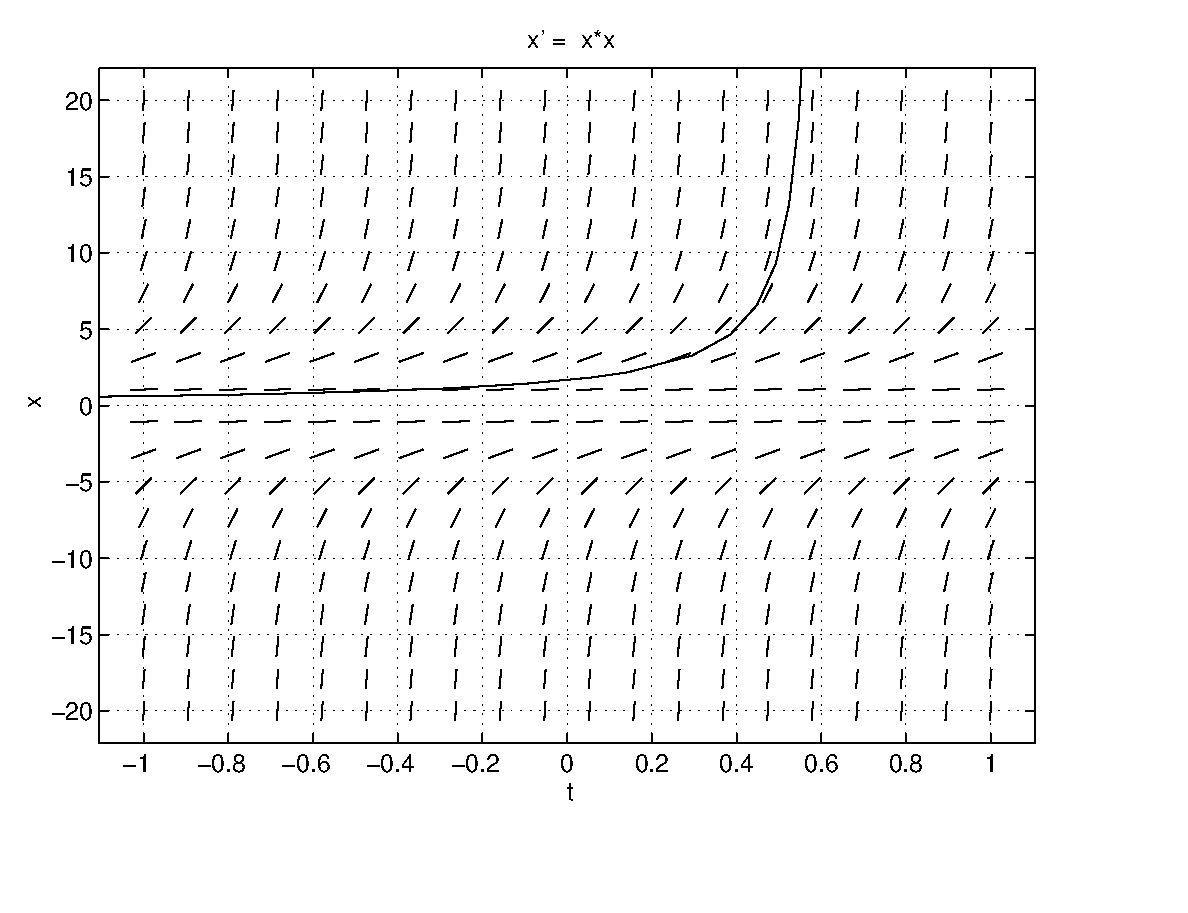
\psfig{file=../figures/x2a.eps,width=3.5in}
	   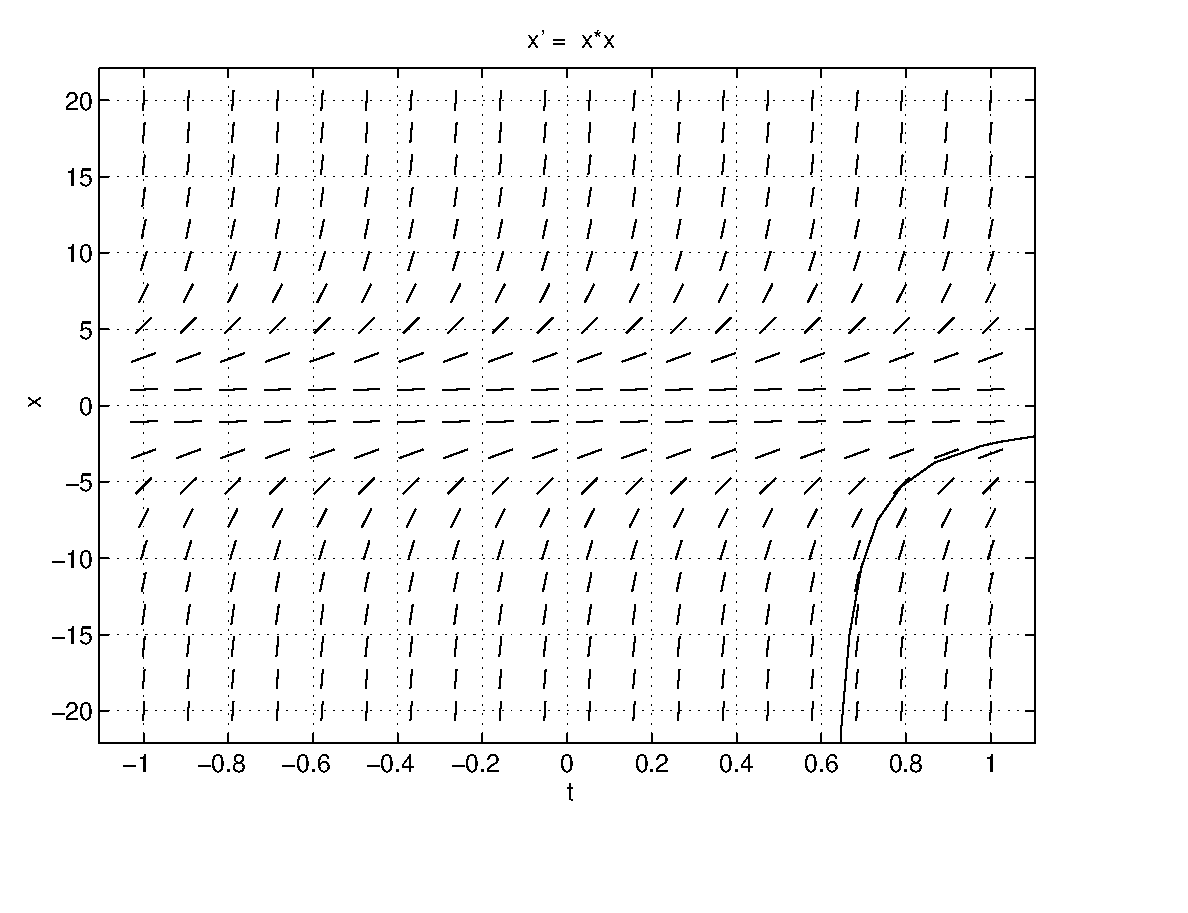
\psfig{file=../figures/x2b.eps,width=3.5in}}
           \caption{Solutions using {\sf dfield5} for $\frac{dx}{dt} = x^2$ 
		with initial conditions: (left) $(x_0,t_0)=(2,0.1)$ and 
		(right) $(x_0,t_0)=(1,-2.5)$.}
           \label{F:x^2}
\end{figure*}

\subsubsection*{An Example that Cannot be Solved in Closed Form}

Consider the differential equation
\begin{equation}  \label{E:ncf}
\frac{dx}{dt} = \frac{x}{x-1}
\end{equation}
with initial condition $x(1)=2$. On division \Ref{E:ncf} becomes 
\[
\left(1-\frac{1}{x}\right)\frac{dx}{dt} = 1.
\]
Integration with respect to $t$ yields
\[
x - \ln|x| = t + C.
\]
Using the initial condition, we see that 
\[
C = 2 - \ln 2 -1 = 1 - \ln 2.
\]
Note that for $t$ near $1$, the initial condition implies that $x(t)>0$.  
Hence $x(t)$ satisfies
\begin{equation} \label{e:solnncf}
x -\ln x = t + 1 - \ln 2.
\end{equation}
Unfortunately, this equation cannot be solved explicitly for $x$ 
as a function of $t$; that is, there is no closed form 
solution\index{closed form solution} 
for $x(t)$.  Nevertheless, $x(t)$ is defined 
{\em implicitly\/}\index{solution!implicitly defined} 
by \Ref{e:solnncf}.  This equation can, however, be solved numerically by
{\sf dfield5} just as easily as equations that have closed form solutions.
See Exercise~\ref{c14.1.17}. 

\subsection*{The General Solution by Separation of Variables}
\index{separation of variables!general solution}

The solution to the initial value problem for the separation
of variables equation
\begin{equation}  \label{eq:ghivp}
\dps \frac{dx}{dt} =  g(x) h(t),
\end{equation}
where $x(t_0) = x_0$, is obtained by combining the integrations of the two 
special cases just considered.  

Note that if $g(x_0)=0$, then $x(t)=x_0$ is an equilibrium solution to 
\Ref{eq:ghivp}.  So we can assume 
\begin{equation} \label{eq:gx0}
g(x_0)\not=0,
\end{equation}
and divide \Ref{eq:ghivp} by $g(x)$ to obtain
\[
\frac{1}{g(x)}\frac{dx}{dt}= h(t).
\]
Integrating with respect to $t$ yields
\[
\int \frac{1}{g(x)} \frac{dx}{dt}dt = \int h(t) dt + C.
\]
As before, on changing variables, we obtain
\[
\int\frac{1}{g(x)} dx = \int h(t) dt.
\]
Thus, the abstract solution to \Ref{eq:ghivp} can be written as
\begin{equation} \label{E:G=H+K}
G(x) = H(t) + C,
\end{equation}
where $G$ is an indefinite integral of $1/g$ and $H$ is an indefinite 
integral of $h$, and 
\begin{equation}  \label{E:G=H+Kinit}
C = G(x_0)-H(t_0).
\end{equation}



\subsubsection*{An Example Solving the Initial Value Problem}
\index{separation of variables!initial value problem}

We illustrate the technique of separation of variables with the following
example.  Find the solution of the initial value problem
\[
\frac{dx}{dt} = \frac{t}{x^2} 
\]
where $x(1)=2$.  Here $g(x) = 1/x^2$ and $h(t) = t$, so that
\[
G(x)=\int x^2 dx= \frac{1}{3}x^3 \AND H(t) = \int t dt = \frac{1}{2}t^2.
\]
Since $t_0=1$ and $x_0=2$, we can use \Ref{E:G=H+Kinit} to see that 
\[
C = G(2)-H(1) = \frac{8}{3} -\frac{1}{2} = \frac{13}{6},
\]
and \Ref{E:G=H+K} to see that the solution $x(t)$ satisfies
\[
\frac{1}{3}x(t)^3 = \frac{1}{2}t^2 + \frac{13}{6}.
\]
Therefore,
\[
x(t) = \left(\frac{3t^2+13}{2}\right)^{1/3}.
\]
The reader may check that this function is indeed a solution
satisfying the specified initial condition.

\subsubsection*{An Example Finding a General Solution}
\index{separation of variables!general solution}

With this example, we illustrate how to use separation of variables to find 
all solutions of a differential equation in the form \Ref{eq:gh}.  Consider
\begin{equation} \label{eq:x1t2}
\frac{dx}{dt} = \frac{(x+1)(t^2+1)}{t}
\end{equation}
for $t>0$.  Using our notation we have 
\[
g(x) = x+1 \AND h(t) = t+\frac{1}{t}.
\]
Note that $g(-1)=0$ and hence that $x(t)=-1$ is the constant equilibrium 
solution to \Ref{eq:x1t2}.  For all the other initial conditions, we obtain 
\[
G(x)=\int \frac{1}{x+1} dx = \ln|x+1| \AND 
H(t) = \int\left(t + \frac{1}{t}\right)dt = \frac{1}{2}t^2 + \ln |t|.
\]
Thus, in this example, identity \Ref{E:G=H+K} implies that the 
solution $x(t)$ satisfies
\[
\ln |x(t)+1| = \frac{1}{2}t^2 + \ln |t| + C.
\]
Hence
\[
|x(t)+1| = K|t|e^{t^2/2},
\]
for some constant $K>0$ and nonconstant solutions of \Ref{eq:x1t2} are in 
one-to-one correspondence with functions
\[
x(t) = Kte^{t^2/2}-1
\]
for $K\in\R$.  Note that setting $K=0$ recovers the constant solution 
$x(t)=-1$.

\EXER

\TEXER

\noindent In Exercises~\ref{c14.1.1a} -- \ref{c14.1.1d} decide whether 
or not the method of separation of variables can be applied to the given
differential equation.  If this method can be applied, then specify the 
functions $g$ and $h$ --- but do not perform the integrations.
\begin{exercise} \label{c14.1.1a}
$\dps \frac{dx}{dt} = x^{1/2}\cos t$.
\end{exercise}
\begin{exercise} \label{c14.1.1b}
$\dps \frac{dx}{dt} = (x+xt)\tan x$.
\end{exercise}
\begin{exercise} \label{c14.1.1c}
$\dps \frac{dx}{dt} = (x+t)(x-t)$.
\end{exercise}
\begin{exercise} \label{c14.1.1d}
$\dps \frac{dx}{dt} = 3-2x+3t-2xt$.
\end{exercise}

\noindent In Exercises~\ref{c14.1.5a} -- \ref{c14.1.5c} solve the given 
initial value problem by separation of variables. 
\begin{exercise}  \label{c14.1.5a}
$\dps \frac{dx}{dt} = -3x,\quad x(0)=-1.$
\end{exercise}
\begin{exercise}  \label{c14.1.5b}
$\dps \frac{dx}{dt} = \frac{t^3-1}{\cos x},
\quad x(\pi)=\frac{\pi}{2}.$
\end{exercise}
\begin{exercise}  \label{c14.1.5c}
$\dps \frac{dx}{dt} = 2\sqrt{tx},\quad x(1)=1.$
\end{exercise}

\noindent In Exercises~\ref{c14.1.8a} -- \ref{c14.1.8c} use separation 
of variables to find all the solutions of the given differential equation.
\begin{exercise}  \label{c14.1.8a}
$\dps \frac{dx}{dt} = 2x$.
\end{exercise}
\begin{exercise}  \label{c14.1.8b}
$\dps \frac{dx}{dt} = 5x+2$.
\end{exercise}
\begin{exercise}  \label{c14.1.8c}
$\dps \frac{dx}{dt} = \frac{\sin t}{x}$.
\end{exercise}

\CEXER

\noindent We have studied the autonomous linear differential equation 
$\dot{x}=\lambda x$ when $\lambda\neq 0$ and have shown that solutions 
exist for all time and tend either to $0$ or to $\pm\infty$ as $t\to\pm\infty$.
See \Ref{explimits} and Figure~\ref{df_dsp1}.  In Exercises~\ref{c14.1.11a} -- 
\ref{c14.1.11f} explore the behavior of solutions $x(t)$ of the given 
nonlinear (and often nonautonomous) differential equation using {\sf dfield5}.  
Where possible, describe the differences between the behavior of solutions of 
the given differential equation and the linear differential equation.  

\noindent{\bf Hint:}  Here is a list of properties of solutions that are 
{\em not valid\/} for solutions to the linear differential equation:
\begin{itemize}
\item[(a)]  Solutions blow up in finite time (that is, 
$\lim_{t\to t_0}x(t)=\pm\infty$).
\item[(b)]  Solutions do not exist for all time.
\item[(c)]  Multiple solutions are bounded in both forward and backward time.
(In the linear system only the zero solution $x(t)=0$ is bounded in both 
forward and backward time.)
\item[(d)]  Solutions stop (that is, solutions limit in either forward or 
backward time on a finite value of $x$ in finite time $t$).
\end{itemize}
Use {\sf dfield5} to determine which of these properties of solutions are 
valid for the given differential equations.  Also, when exploring 
Exercises~\ref{c14.1.11a} -- \ref{c14.1.11f} be prepared to use the {\sf Stop}
button in the {\sf DFIELD5 Display} window to stop the numerical integration. 

\begin{exercise} \label{c14.1.11a}
$\dps\frac{dx}{dt} = \frac{1}{x}$.
\end{exercise}
\begin{exercise} \label{c14.1.11b}
$\dps\frac{dx}{dt} = \frac{1}{tx}$.
\end{exercise}
\begin{exercise} \label{c14.1.11c}
$\dps\frac{dx}{dt} = \sin(tx)$.
\end{exercise}
\begin{exercise} \label{c14.1.11d}
$\dps\frac{dx}{dt} = t^2 - x^3$.
\end{exercise}
\begin{exercise} \label{c14.1.11e}
$\dps\frac{dx}{dt} = x(1-x^2)$.
\end{exercise}
\begin{exercise} \label{c14.1.11f}
$\dps\frac{dx}{dt} = \frac{t}{x^2}$.
\end{exercise}

\begin{exercise} \label{c14.1.17}
Recall that the differential equation \Ref{E:ncf} $\dot{x}=x/(x-1)$ cannot be 
solved in closed form.  
\begin{itemize}
\item[(a)]	Use {\sf dfield5}\index{\computer!dfield5} 
to solve this differential 
equation numerically on the interval $0.8\leq t\leq 1.2$ with initial 
condition $x(1)=2$.  (Set the $x$ interval to be $[0,4]$.)  
\item[(b)]	Using this result estimate the value of $x(1.15)$ to two 
decimal places.
\item[(c)]	Next change the time interval to be $0.5\leq t\leq 1.2$.
The numerically computed solution $x(t)$ behaves strangely when $t\leq 0.7$. 
What is the approximate value of $x$ in this range of $t$?  Use this 
observed value to explain why the numerical integration for this differential 
equation is badly behaved.
\end{itemize}
\end{exercise}

\begin{exercise} \label{c14.1.18}
The ability to find closed form solutions to differential equations enables
us to test the accuracy of numerically computed solutions.  As an example where difficulties arise in numerical computations, consider the differential 
equation
\begin{equation} \label{eq:exivp}
\frac{dx}{dt} = \left(\frac{x}{t}\right)^2.
\end{equation}
\begin{itemize}
\item[(a)] Use separation of variables to find the solution $x(t)$ to the 
initial value problem $x(0.001) = 2/1999$ of \Ref{eq:exivp}.
\item[(b)] Show that $\dps\lim_{t\to 2^-}x(t)=\infty$ for the solution of 
\Ref{eq:exivp} obtained in (a).
\item[(c)] For the initial condition specified in (a) compare the analytic 
solution of \Ref{eq:exivp} to the numerical solution computed by {\sf dfield5} 
in the region where the maximum value of $t$ is $2.5$ and the maximum value of 
$x$ is $100$.  How does the behavior of the numerically computed solution 
to \Ref{eq:exivp} differ from that of the analytically computed solution?
\item[(d)]  Compute the solution of \Ref{eq:exivp} using the general initial 
condition $x(t_0) = x_0$ where $t_0,x_0>0$ and show that 
$\lim_{t\to 0^+}x(t)=0$ for every such solution. 
\end{itemize}
\noindent {\bf Comment:} Part (d) hints at why there is a discrepancy 
between the numerically approximated solution and the analytic solution: 
small errors in the approximate solution with initial condition $(t_0,x_0)$ 
near $(0,0)$ cause different solutions to be computed.
\end{exercise}

 

\end{document}
